\chapter{System Design with User Perspective}

\newpage

% 1. Model-View-Control
% https://www.youtube.com/watch?v=Y3XKomLAmYI
% https://www.techopedia.com/definition/3842/model-view-controller-mvc

% 2. change presentation language dynamically
% https://stackoverflow.com/questions/46008760/how-to-build-multiple-language-website-using-pure-html-js-jquery

% 3. drag and drop
% https://www.w3docs.com/learn-javascript/drag-and-drop-with-javascript.html
% https://www.youtube.com/watch?v=Wtrin7C4b7w

% 4. Undo-Redo
% save a stack of what items that is being saved

% 5. responsive design
% there is a Device Mode in developer tools for chrome and firefox
% https://www.youtube.com/watch?v=ZYV6dYtz4HA

\begin{multicols}{2}
\section{Documentation}
\begin{itemize}
\item One of the most important things in life is to understand...
\item I want you to understand WHY you need to document a program!
\item Then the HOW becomes much easier!
\end{itemize}

\begin{itemize}
\item The documentation is the user interface to the program code!
\item It is possible to work without it, but who want to code in assembler?
\end{itemize}

\subsection{Implicit documentation}
\begin{itemize}
\item Names can tell a story (meaningful names)
\item Names can also be classifying the variable (x,y positions. i,j,k index)
\item Choose the right algorithms and data structures
\end{itemize}


\subsection{Implicit documentation}
\begin{itemize}
\item Several diffrent versions of documetation
  \begin{itemize}
  \item Meta documentation (Each file: Discription, author, protocols, file dependencies)
  \item External document (Manuals/Installation instruction, list of tree structures)
  \item Inline documentation (Difficult code, TODO)
  \end{itemize}
\end{itemize}


\section{Human factors}
\subsection{Color combinations}
There are some color combinations with humans have difficulty prossessing on of with is
Red text on Blue backround and Blue text on red backround.

\subsection{Personas}
Who are the real people who will use this program. With that information mace sure it
is well suted for them and there needs as well as for there difficulties.

\subsection{Memory}
Our memory is like a net wire eatch connection is from one peace of information to another
there for memory needs to be assosiated with the nessesary areas. For instance when we
design a web shop we should have the checkout on the right top since for most web shops have
that and therfore people make that connection that this is a web shop there fore the checkout
is on the top right.

\subsection{What is needed to desing a system?}
\begin{itemize}
\item Requirement specification
\item Specify in detail the requirements on the software
  \begin{itemize}
  \item What should it be able manage?
    \begin{itemize}
    \item Number of customers, number of items in store, etc.
    \end{itemize}
  \item Which functions are needed?
  \end{itemize}
\item Order a beverage, check stored items, etc.
\end{itemize}

\section{Model-View-Control}
Initially a Object-Oriented (interface) Design model.
Purpose: Making the View separated from the Mode.

\begin{figure}[h]
    \vspace{10mm}
    \centering
    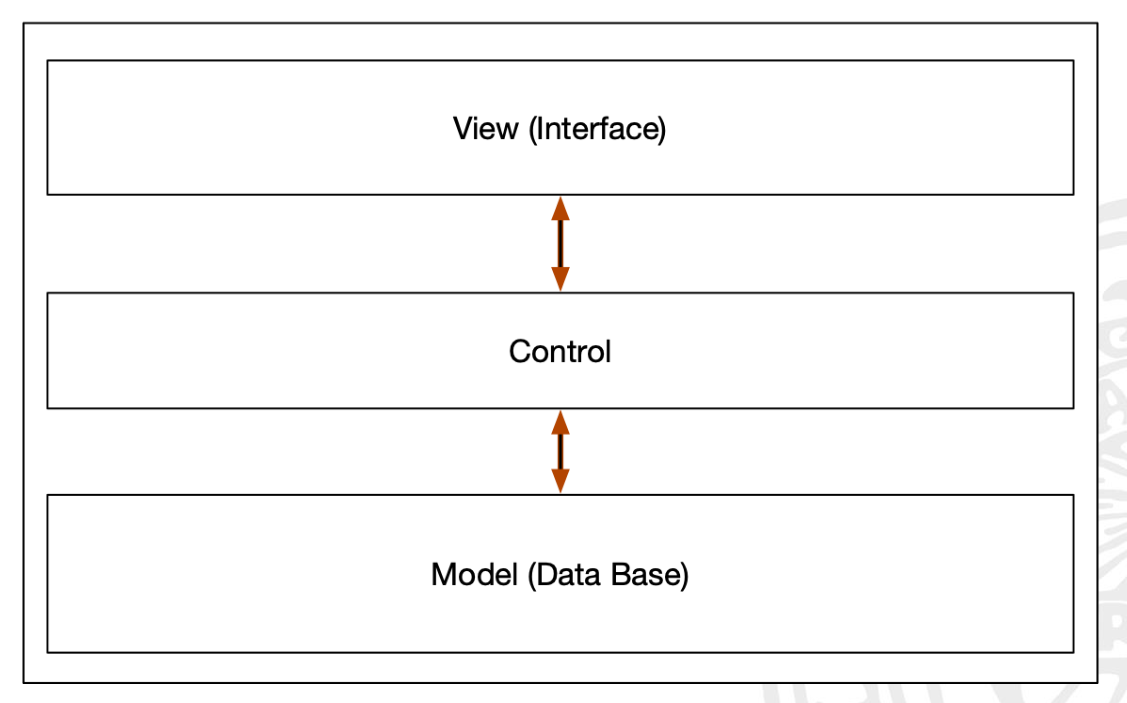
\includegraphics[width=10cm, height=5cm]{image/mvc.png}
    \caption{MVC}
\end{figure}

\begin{itemize}
\item View is only presentation of a Designed Interaction!
\item Start by modelling the Model and Control (as a command Interface)
\item Then implement the View (both control and presentation).
  \begin{itemize}
  \item Create a good metaphor to the things that happen in
  \end{itemize}
\end{itemize}

\end{multicols}